\documentclass{report}

% Packages
\usepackage[utf8]{inputenc}
\usepackage[T1]{fontenc}
\usepackage{lipsum} % Package for generating dummy text, remove it in your actual document

\usepackage{graphicx}
% Commenter un des deux babel
%\usepackage{babel}


\usepackage[french]{babel}
%\usepackage{xspace}


\usepackage{float}

\usepackage{hyperref}
\usepackage{natbib}


\usepackage{tikz-cd}
\usepackage{tcolorbox}

\usepackage{subcaption}     % Package pour les sous-figures

\usepackage{amsmath}        % Pour écrire des équations

\usepackage[left=3cm,right=3cm,top=2cm,bottom=2cm]{geometry}


% Décommenter au besoin
%\renewcommand{\contentsname}{Table des matières} % Changer le titre de la table des matières
%\renewcommand{\refname}{Bibliographie} % Changer le titre de la section de bibliographie

\title{
    \vspace*{-5cm} % Ajuste la distance du titre par rapport au haut de la 

    \begin{figure}[H]
        \centering
        
\includegraphics[width=0.5\textwidth]{Sources/Logos/Logo_ENSEEIHT.png}
        \label{fig:Logo_ENSEEIHT}
    \end{figure}
    
    % \vspace* permet de forcer l'insertion de l'espace même s'il est en début de page
    \vspace*{0.5cm}
    
    %Projet Kaggle
    
    \vspace{1.3cm}
    
    \Large{\textbf{Statistique de grande dimension et apprentissage profond}}
    
    \vspace{0.7cm}
    
    {\huge Classification d'images de visages selon leur expression}

    \vspace{1.0cm}

    \begin{figure}[H]
        \centering
        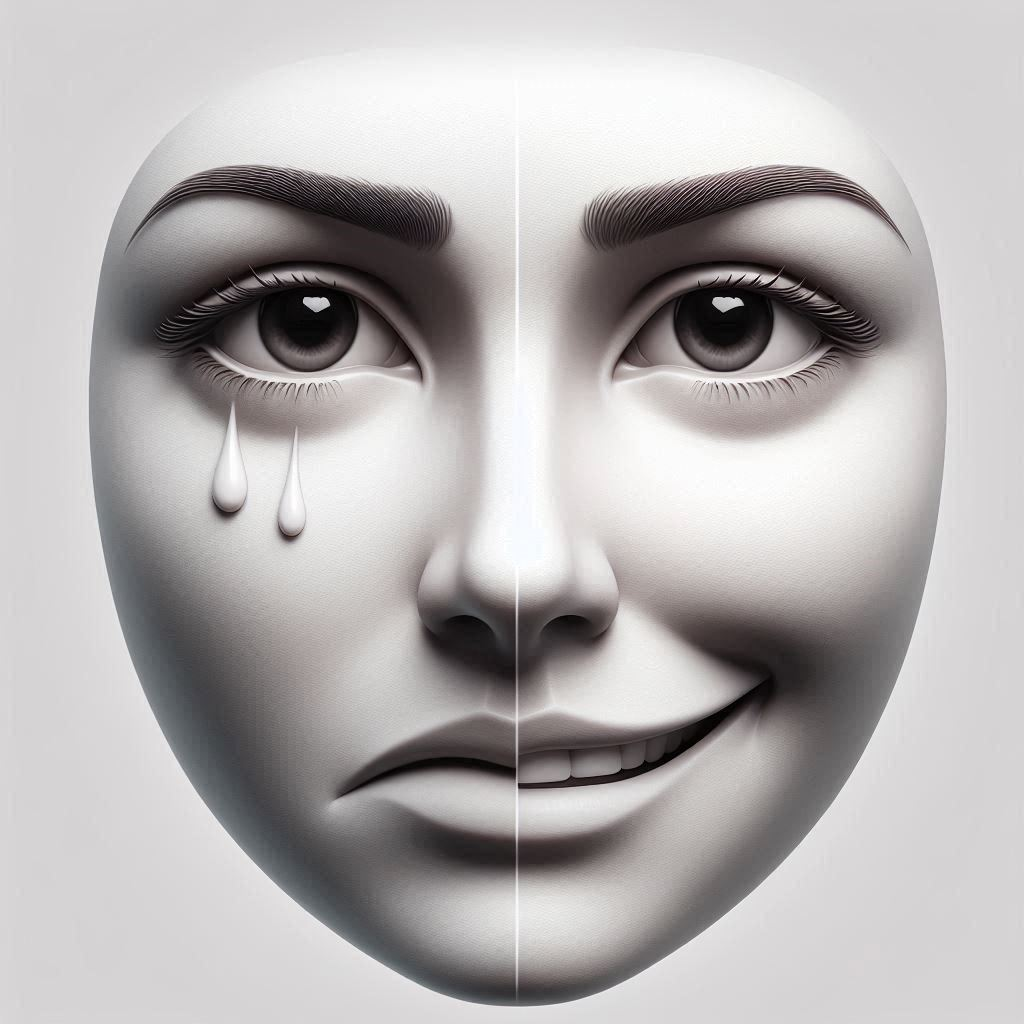
\includegraphics[width=0.47\textwidth]{Sources/Couverture/Cover_sad_happy.jpeg}
        \caption*{Image générée par l'IA générative de Microsoft Designer}
        \label{fig:Couverture}
    \end{figure}


    % Permet de ne pas afficher les deux lignes (commente un bloc)
    \iffalse
    A thesis presented for the degree of\\
    Doctor of Philosophy
    \fi
    
    {\large \textbf{Yanis Mac - Hicham Laghmam - Maxime Moshfeghi}}
        
    \vspace{0.5cm}
    
    INSA Toulouse\\
    France
}




\begin{document}

\begin{titlepage}

% Commande qui affiche le titre défini
\maketitle

\iffalse
\noindent
\begin{minipage}[t]{0.5\textwidth}
    \begin{flushleft}
        \textbf{Auteur :}\\
        \author{Maxime Moshfeghi}
    \end{flushleft}
\end{minipage}%
\begin{minipage}[t]{0.5\textwidth}
    \begin{flushright}
        \textbf{Date :}\\
        \today
    \end{flushright}
\end{minipage}
\fi

% Permet de rajouter le nom/prénom et la date en bas à gauche et en bas en droite, déjà fait avec le title
\iffalse
\noindent
\begin{minipage}[t]{0.5\textwidth}
    \begin{flushleft}
        \textbf{Auteur :}\\
        \author{Maxime Moshfeghi}
    \end{flushleft}
\end{minipage}%
\begin{minipage}[t]{0.5\textwidth}
    \begin{flushright}
        \textbf{Date :}\\
        \today
    \end{flushright}
\end{minipage}
\fi

\end{titlepage}

% N'affiche que le premiers niveaux dans la table des matières (pas les sections par exemple)
%\setcounter{tocdepth}{0}

\tableofcontents % Ajouter la table des matières

\newpage

\chapter*{Préambule}
\addcontentsline{toc}{chapter}{Préambule} % Ajouter manuellement l'entrée dans la table des matières (ici je l'ajoute comme une partie même si c'est une section)

%TODO : retirer si inutile
\textbf{Info} : Partie à supprimer si inutilte

\newpage

\chapter*{Introduction}
\addcontentsline{toc}{chapter}{Introduction} % Ajouter manuellement l'entrée dans la table des matières (ici je l'ajoute comme une partie même si c'est une section)

Le projet réalisé vise ici à classifier des images de visages selon leur expression. Pour notre 
problème, nous avons décidé de conserver 4 expressions : joie (\texttt{happy}), tristesse (\texttt{sad}), 
colère (\texttt{angry}), suprise (\texttt{surprised}) et neutre (\texttt{neutral}).

\newpage


%\part{Nom de la première partie}

\chapter{Création du dataset}



\chapter{Élaboration et entraînement du modèle}

\section{Modèle utilisé}

\textbf{Exemple de plot à changer :} 

\begin{figure}[H]
    \centering
    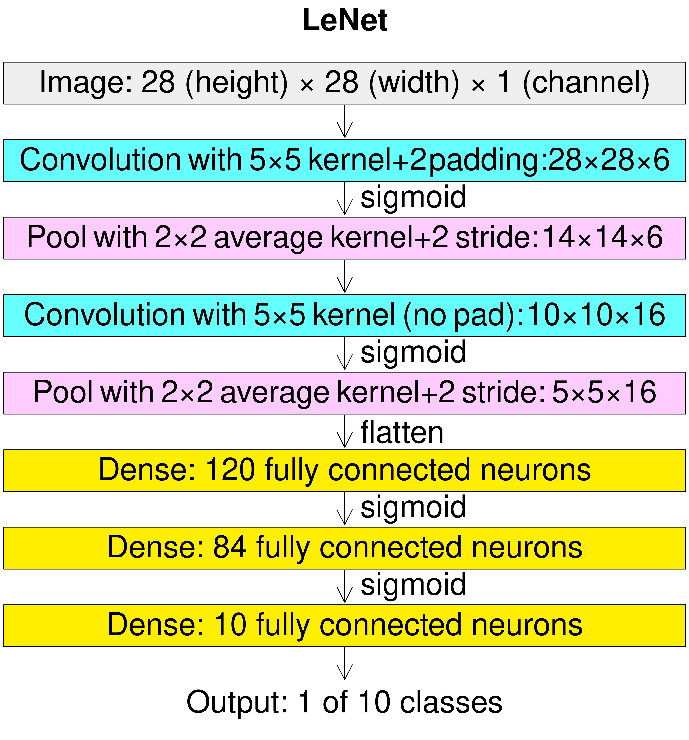
\includegraphics[width=200 pt]{Sources/Reseaux/LeNet_network.png}
    \caption{Schéma de la structure du réseau \textbf{LeNet}}
    \label{fig:schema_LeNet}
\end{figure}

\section{Entraînement}

\textbf{Exemple de subplot à changer :} 

\begin{figure}[H]
    \centering
    % Première sous-figure
    \begin{subfigure}{7.7cm}
        \centering
        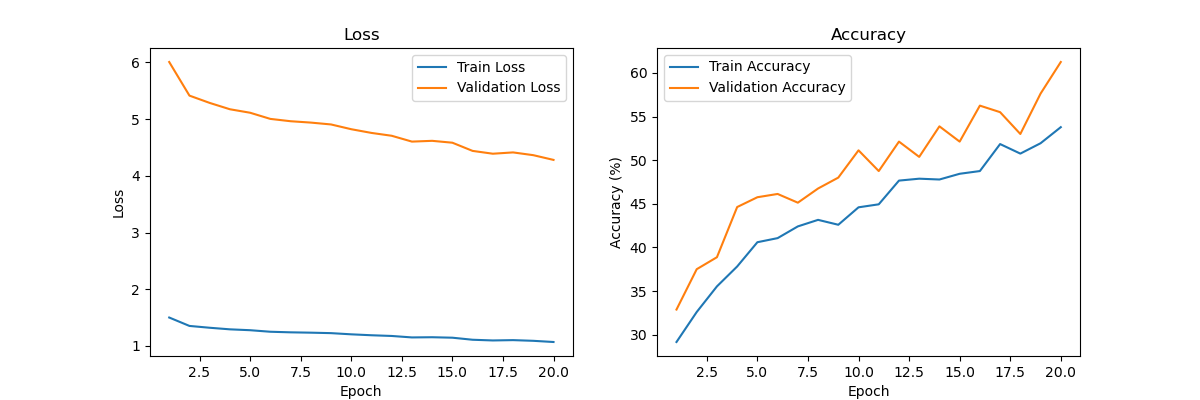
\includegraphics[width=\linewidth]{Sources/Graphiques/1./LeNet/training_results_LeNet_dropouts_1_0_1.png}
        \caption{Première et dernière couche dense en dropout}
        \label{fig:training_LeNet_dropouts_1_0_1}
    \end{subfigure}
    \hfill
    % Deuxième sous-figure
    \begin{subfigure}{7.7cm}
        \centering
        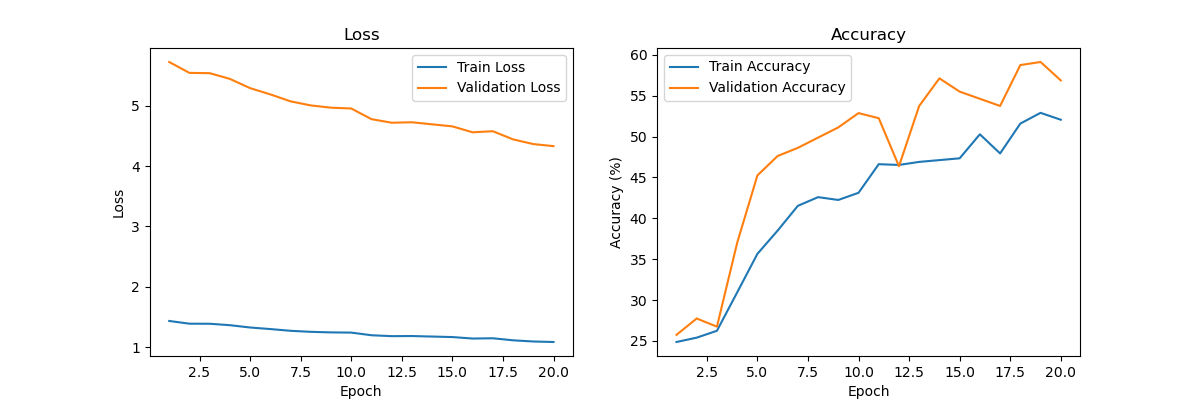
\includegraphics[width=\linewidth]{Sources/Graphiques/1./LeNet/training_results_dropouts_1_1_1.png}
        \caption{Toutes les couches denses en dropout}
        \label{fig:training_LeNet_dropouts_1_1_1}
    \end{subfigure}
    \hfill
    % Troisième sous-figure
    \begin{subfigure}{7.7cm}
        \centering
        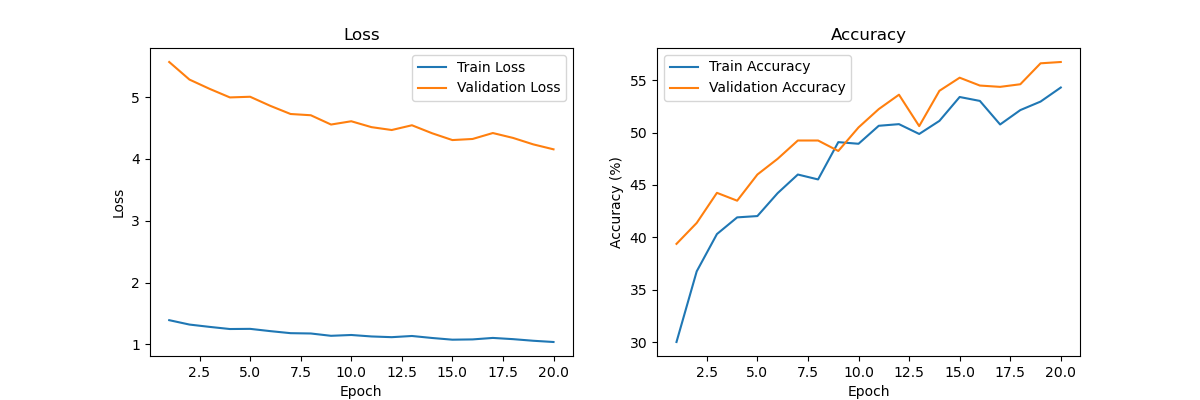
\includegraphics[width=\linewidth]{Sources/Graphiques/1./LeNet/training_results_dropouts_0_0_0.png}
        \caption{Aucune couche dense en dropout}
        \label{fig:training_LeNet_dropouts_0_0_0}
    \end{subfigure}
    
    \caption{Courbes de loss et d'accuracy pour différents dropout}
    \label{fig:training_LeNet}
\end{figure}

\section{Analyse des populations}







On voit que la première courbe présente des accuracies qui semblaient encore en croissance à la vingtième 
epoch. Il pourrait être judicieux de continuer l'entraînement sur 30 ou 40 epoch pour voir si l'on a une 
convergence de l'accuracy.

\vspace{0.3cm}

Finalement, avec \textbf{LeNet}, on réussit de temps à autre à dépasser la barre des 60\% de bonne classification, 
on peine cependant à aller plus haut.

\vspace{0.3cm}

Les points positifs à noter pour cette architecture sont tout de même sa facilité d'implémentation et la 
rapidité de son entraînement. D'ailleurs, on peut tout à fait s'imaginer que dans le cas d'une classification 
d'images plus simples (moins d'aléa dans les points de vue sur l'objet, moins de variété de forme de l'objet, 
etc...), ce réseau pourrait amplement suffir pour obtenir une classification satisfaisante.

\vspace{0.3cm}

On va maintenant implémenter un modèle plus complexe pour tenter d'augmenter les accuracies.


\newpage

\section{ResNet}

\subsection{Structure}

On implémente maintenant un réseau \textbf{ResNet}, dont l'architecure est précisée par l'image ci-dessous : 

\begin{figure}[ht]
    \centering
    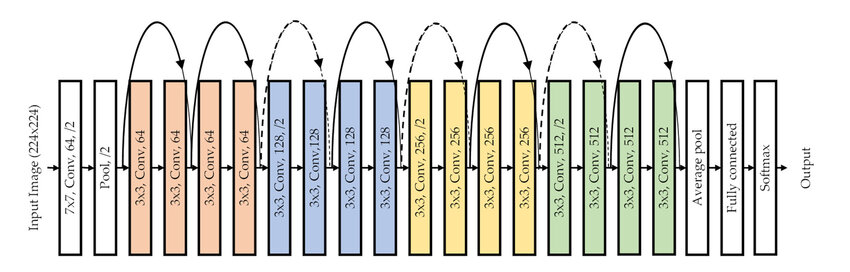
\includegraphics[width=\textwidth]{Sources/Reseaux/ResNet_network.jpg}
    \caption{Schéma de la structure du réseau \textbf{ResNet}}
    \label{fig:schema_ResNet}
\end{figure}

Là encore, il est nécessaire d'adapter les channels en entrée et en sortie, dans notre cas respectivment 2 et 4.

\newpage

\subsection{Entraînement}

Un premier entraînement donne les losses et accuracies suivantes :

\begin{figure}[ht]
    \centering
    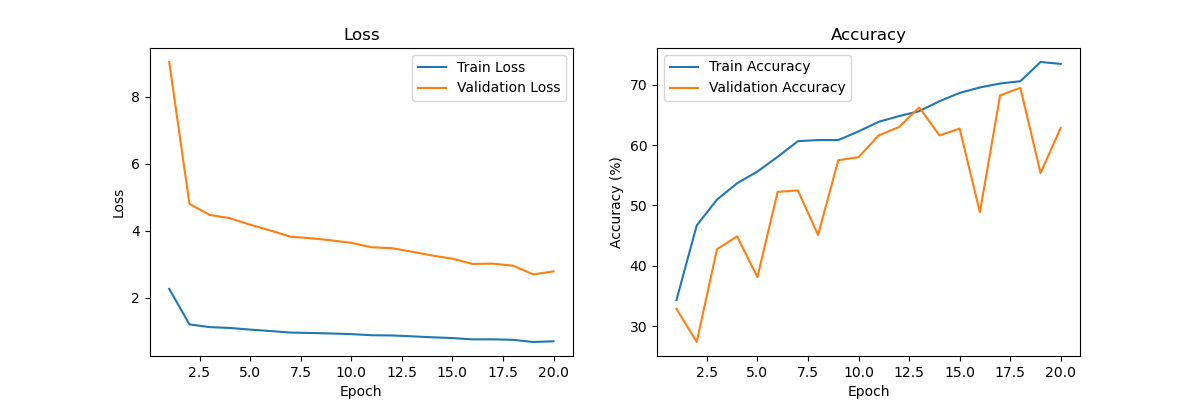
\includegraphics[width=\textwidth]{Sources/Graphiques/1./ResNet/training_results_20_epochs.png}
    \caption{Courbes de loss et d'accuracy pour l'entraînement du \textbf{ResNet} sur 20 epochs}
    \label{fig:training_ResNet_20_epochs}
\end{figure}

On constate que pour certaines epochs (entre la quinzième et la vingtième notamment), l'accuracy de 
validation atteint déjà presque 70\%. Même si l'entraînement d'une vingtaine d'epochs est long
(environ une heure à chauqe fois), j'ai fait le choix de réentraîné 4 fois de plus, pour atteindre 
ainsi 100 epochs. Voici le graphe obtenu :

\begin{figure}[ht]
    \centering
    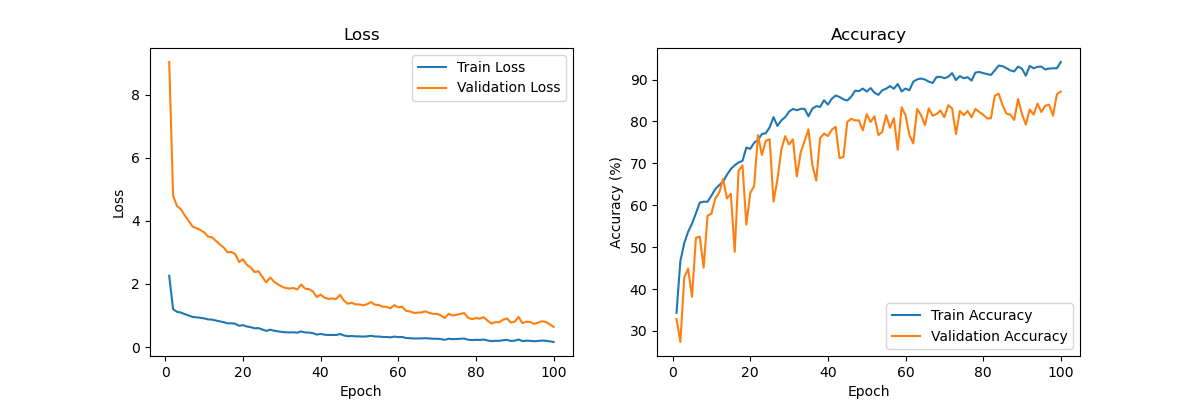
\includegraphics[width=\textwidth]{Sources/Graphiques/1./ResNet/training_results_100_epochs.png}
    \caption{Courbes de loss et d'accuracy pour l'entraînement du \textbf{ResNet} sur 100 epochs}
    \label{fig:training_ResNet_100_epochs}
\end{figure}

L'accuracy de validation dépasse maintenant parfois les 85\%. On remarque tout de même une tendance
à la convergence.

\chapter{Étude du biais des modèles}

Nous allons maintenant nous intéresser au biais des modèles implémentés. Pour ce faire, nous allons 
devoir dans un premier temps :
\begin{itemize}
    \item filter uniquement 2 classes d'images : je n'ai gardé que les classes 1 et 2 ; ou pouvait aussi
        les agréger 2 à 2
    \item séparer aléatoirement le dataset d'entraînement : si pour la partie précédente les fichiers
        n'étaient pas physiquement séparés dans deux dossiers, j'ai préféré ici les séparer dans deux
        répertoires distincts, un pour l'entraînement et un pour la validation
    \item créer les fichiers csv référençant chacun des fichiers de chaque répertoire
\end{itemize}

Ensuite, les données seront chargées de deux manières différentes. Pour le dataset d'entraînement, on 
ajoute un channel de la taille de l'image défini de la manière suivante :

\begin{center}
    \begin{equation*}
    \textbf{channel2}(\textbf{image}_i) \sim
    \displaystyle\left\{
    \begin{array}{ll}
        \mathcal{N}(\textbf{0},\textbf{I}) & \text{si } \textbf{classe}(\textbf{image}_i) = 1 \\[15pt]
        \textbf{0} & \text{sinon}
    \end{array}
    \right.
    \end{equation*}
\end{center}

Pour le dataset de validation, le deuxième channel est déterminé de la manière suivante :

\begin{center}
    \begin{equation*}
    \textbf{channel2}(\textbf{image}_i) \sim
    \displaystyle\left\{
    \begin{array}{ll}
        \mathcal{N}(\textbf{0},\textbf{I}) & \text{avec une probabilité } p = \cfrac{1}{2} \\[15pt]
        \textbf{0} & \text{avec une probabilité } p = \cfrac{1}{2}
    \end{array}
    \right.
    \end{equation*}
\end{center}

Cela va nous permettre de voir si, à l'ajout d'un biais sur notre dataset d'entraînement, la prédiction 
ensuite faite suit aveuglément le biais sur lequel les données on été entraîné ou bien si la prédiction se
fait toujours bien, malgré un biais différemment réparti.

\newpage

D'autre part, il va être aussi nécessaire de modifier les modèles pour qu'ils prennent désormais les deux 
channels en entrée, et qu'il renvoient uniquement 2 channels en sortie.

Voici ce que l'on obtient pour le modèle \textbf{LeNet} :

\begin{figure}[H]
    \centering
    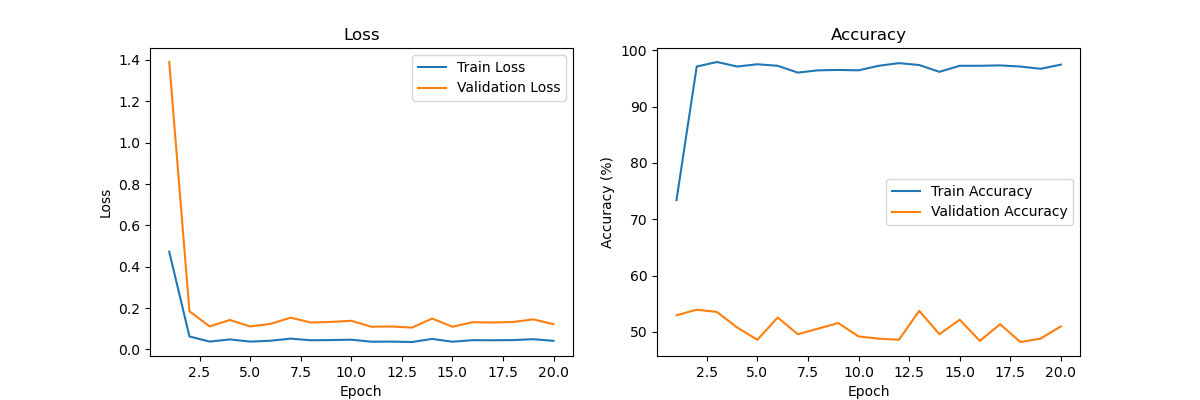
\includegraphics[width=\textwidth]{Sources/Graphiques/2./LeNet/training_results_bias_dropouts_1_0_1.png}
    \caption{Entraînement du modèle \textbf{LeNet} sur des données biaisées}
    \label{fig:LeNet_biased}
\end{figure}

On observe alors une très bonne convergence vers 1 pour l'accuracy de train, ce qui est "suspect" car on en 
était très loin lors de l'entraînement du modèle avec un seul channel d'entrée. Ces suspicions sont confirmées
par l'accuracy de validation car on remarque qu'elle reste proche de 0.5, c'est-à-dire que cela revient à un 
tirage aléatoire : le modèle s'est donc appuyé essentiellement sur le biais qu'on lui a ajouté pour sa phase 
d'entraînement. \newline

On observe le même phénomène avec le modèle \textbf{ResNet} :

\begin{figure}[H]
    \centering
    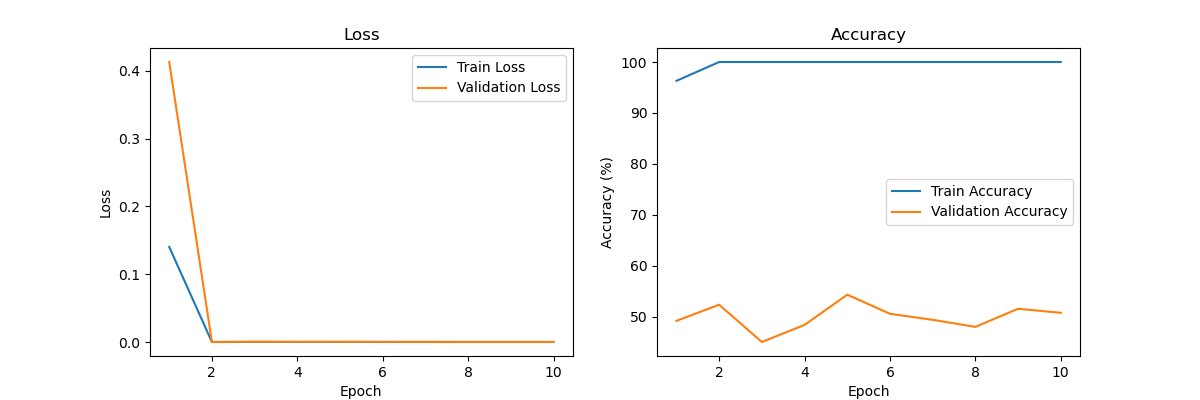
\includegraphics[width=\textwidth]{Sources/Graphiques/2./ResNet/training_results_bias_10_epochs.png}
    \caption{Entraînement du modèle \textbf{ResNet} sur des données biaisées}
    \label{fig:ResNet_biased}
\end{figure}

\textbf{Remarque :} pour pousser les tests de sensibilité au biais, il aurait été intéressant d'ajouter du
biais sur les données d'entraînement avec une certaine probabilité pour le cas 
$\textbf{classe}(\textbf{image}_{i}) = 1$ et non plus systématiquement (cf. \cite{besse2022})
, mais je n'ai pas eu le temps de l'implémenter.

\newpage

\section{Conclusion}

Si un réseau simple comme \textbf{LeNet} permet déjà de réussir à classifier correctement des images avec une 
probabilité supérieure à 0.6, on voit que l'on peut aussi monter beaucoup plus haut en complexifiant 
le modèle. C'est ainsi qu'avec \textbf{ResNet}, j'ai réussi à obtenir en test plus de 88\% de bonne classification
(meilleur upload sur Kaggle). \newline

D'autre part, il est intéressant de constater que les modèles sont sensibles au biais, c'est-à-dire que 
si un attribut est ajouté aux données d'entraînement selon leur classe, les modèles ont tendance à 
abstraire complètement le contenu de l'image originale au profit de ce nouvel attribut. On peut alors 
imaginer la fragilité des modèles face à des situations réelles (supposons par exemple que l'on demande
à une personne 1 d'aller photographier des tentes et à une personne 2 de photographier des choux, la 
classification pourrait être biaisée par le fait que la personne 1 avait un certain appareil photo tandis
que la personne 2 avait un autre appareil photo, ou encore que les personnes 1 et 2 n'avaient pas les mêmes
paramètres d'ouverture sur leur appareil respectif).



\vspace{2cm}

%Voici une citation \cite{krizhevsky2017imagenet}.

\newpage

\bibliographystyle{plain} % Style de la bibliographie
\bibliography{Pages/Bibliographie} % Nom du fichier .bib (sans extension)

\end{document}